\documentclass[journal,12pt,twocolumn]{IEEEtran}
\usepackage{setspace}
\usepackage{gensymb}
\usepackage{caption}
%\usepackage{multirow}
%\usepackage{multicolumn}
%\usepackage{subcaption}
%\doublespacing
\singlespacing
\usepackage{csvsimple}
\usepackage{amsmath}
\usepackage{multicol}
%\usepackage{enumerate}
\usepackage{amssymb}
%\usepackage{graphicx}
\usepackage{newfloat}
%\usepackage{syntax}
\usepackage{listings}
\usepackage{color}
\usepackage{tikz}
\usepackage{graphicx}
\usetikzlibrary{shapes,arrows}
\usepackage{chngcntr}
\counterwithin{figure}{section}
%\usepackage{graphicx}
%\usepackage{amssymb}
%\usepackage{relsize}
%\usepackage[cmex10]{amsmath}
%\usepackage{mathtools}
%\usepackage{amsthm}
%\interdisplaylinepenalty=2500
%\savesymbol{iint}
%\usepackage{txfonts}
%\restoresymbol{TXF}{iint}
%\usepackage{wasysym}
\usepackage{amsthm}
\usepackage{mathrsfs}
\usepackage{txfonts}
\usepackage{stfloats}
\usepackage{cite}
\usepackage{cases}
\usepackage{mathtools}
\usepackage{caption}
\usepackage{enumerate}	
\usepackage{enumitem}
\usepackage{amsmath}
%\usepackage{xtab}
\usepackage{longtable}
\usepackage{multirow}
%\usepackage{algorithm}
%\usepackage{algpseudocode}
\usepackage{enumitem}
\usepackage{mathtools}
\usepackage{hyperref}
%\usepackage[framemethod=tikz]{mdframed}
\usepackage{listings}
    %\usepackage[latin1]{inputenc}                                 %%
    \usepackage{color}                                            %%
    \usepackage{array}                                            %%
    \usepackage{longtable}                                        %%
    \usepackage{calc}                                             %%
    \usepackage{multirow}                                         %%
    \usepackage{hhline}                                           %%
    \usepackage{ifthen}                                           %%
  %optionally (for landscape tables embedded in another document): %%
    \usepackage{lscape}     


\usepackage{url}
\def\UrlBreaks{\do\/\do-}


%\usepackage{stmaryrd}


%\usepackage{wasysym}
%\newcounter{MYtempeqncnt}
\DeclareMathOperator*{\Res}{Res}
%\renewcommand{\baselinestretch}{2}
\renewcommand\thesection{\arabic{section}}
\renewcommand\thesubsection{\thesection.\arabic{subsection}}
\renewcommand\thesubsubsection{\thesubsection.\arabic{subsubsection}}

\renewcommand\thesectiondis{\arabic{section}}
\renewcommand\thesubsectiondis{\thesectiondis.\arabic{subsection}}
\renewcommand\thesubsubsectiondis{\thesubsectiondis.\arabic{subsubsection}}

% correct bad hyphenation here
\hyphenation{op-tical net-works semi-conduc-tor}

%\lstset{
%language=C,
%frame=single, 
%breaklines=true
%}

%\lstset{
	%%basicstyle=\small\ttfamily\bfseries,
	%%numberstyle=\small\ttfamily,
	%language=Octave,
	%backgroundcolor=\color{white},
	%%frame=single,
	%%keywordstyle=\bfseries,
	%%breaklines=true,
	%%showstringspaces=false,
	%%xleftmargin=-10mm,
	%%aboveskip=-1mm,
	%%belowskip=0mm
%}

%\surroundwithmdframed[width=\columnwidth]{lstlisting}
\def\inputGnumericTable{}                                 %%
\lstset{
%language=C,
frame=single, 
breaklines=true,
columns=fullflexible
}

\begin{document}
%
\tikzstyle{block} = [rectangle, draw,
    text width=3em, text centered, minimum height=3em]
\tikzstyle{sum} = [draw, circle, node distance=3cm]
\tikzstyle{input} = [coordinate]
\tikzstyle{output} = [coordinate]
\tikzstyle{pinstyle} = [pin edge={to-,thin,black}]

\theoremstyle{definition}
\newtheorem{theorem}{Theorem}[section]
\newtheorem{problem}{Problem}
\newtheorem{proposition}{Proposition}[section]
\newtheorem{lemma}{Lemma}[section]
\newtheorem{corollary}[theorem]{Corollary}
\newtheorem{example}{Example}[section]
\newtheorem{definition}{Definition}[section]
%\newtheorem{algorithm}{Algorithm}[section]
%\newtheorem{cor}{Corollary}
\newcommand{\BEQA}{\begin{eqnarray}}
\newcommand{\EEQA}{\end{eqnarray}}
\newcommand{\define}{\stackrel{\triangle}{=}}
\bibliographystyle{IEEEtran}
%\bibliographystyle{ieeetr}
\providecommand{\nCr}[2]{\,^{#1}C_{#2}} % nCr
\providecommand{\nPr}[2]{\,^{#1}P_{#2}} % nPr
\providecommand{\mbf}{\mathbf}
\providecommand{\der}[1]{\mathrm{d} #1}
\providecommand{\pr}[1]{\ensuremath{\Pr\left(#1\right)}}
\providecommand{\qfunc}[1]{\ensuremath{Q\left(#1\right)}}
\providecommand{\sbrak}[1]{\ensuremath{{}\left[#1\right]}}
\providecommand{\lsbrak}[1]{\ensuremath{{}\left[#1\right.}}
\providecommand{\rsbrak}[1]{\ensuremath{{}\left.#1\right]}}
\providecommand{\brak}[1]{\ensuremath{\left(#1\right)}}
\providecommand{\lbrak}[1]{\ensuremath{\left(#1\right.}}
\providecommand{\rbrak}[1]{\ensuremath{\left.#1\right)}}
\providecommand{\cbrak}[1]{\ensuremath{\left\{#1\right\}}}
\providecommand{\lcbrak}[1]{\ensuremath{\left\{#1\right.}}
\providecommand{\rcbrak}[1]{\ensuremath{\left.#1\right\}}}
\theoremstyle{remark}
\newtheorem{rem}{Remark}
\newcommand{\sgn}{\mathop{\mathrm{sgn}}}
\providecommand{\pd}[2]{\ensuremath{\frac{\partial #1}{\partial #2}}}
\providecommand{\abs}[1]{\left\vert#1\right\vert}
\providecommand{\res}[1]{\Res\displaylimits_{#1}} 
\providecommand{\norm}[1]{\left\Vert#1\right\Vert}
\providecommand{\mtx}[1]{\mathbf{#1}}
\providecommand{\mean}[1]{E\left[ #1 \right]}
\providecommand{\fourier}{\overset{\mathcal{F}}{ \rightleftharpoons}}
\providecommand{\gauss}[2]{\ensuremath{\mathcal{N}(#1, #2)}}
%\providecommand{\hilbert}{\overset{\mathcal{H}}{ \rightleftharpoons}}
\providecommand{\system}{\overset{\mathcal{H}}{ \longleftrightarrow}}
	%\newcommand{\solution}[2]{\textbf{Solution:}{#1}}
\newcommand{\solution}{\noindent \textbf{Solution: }}
\newcommand{\myvec}[1]{\ensuremath{\begin{pmatrix}#1\end{pmatrix}}}
\providecommand{\dec}[2]{\ensuremath{\overset{#1}{\underset{#2}{\gtrless}}}}
\DeclarePairedDelimiter{\ceil}{\lceil}{\rceil}
%\numberwithin{equation}{section}
%\numberwithin{problem}{subsection}
%\numberwithin{definition}{subsection}
\makeatletter
\@addtoreset{figure}{section}
\makeatother
%\let\StandardTheFigure\thefigure
%\renewcommand{\thefigure}{\theproblem.\arabic{figure}}
\renewcommand{\thefigure}{\arabic{section}.\arabic{figure}}
%\numberwithin{figure}{subsection}
%\numberwithin{equation}{subsection}
%\numberwithin{equation}{section}
%\numberwithin{equation}{problem}
%\numberwithin{problem}{subsection}
%\numberwithin{problem}{section}
%%\numberwithin{definition}{subsection}
%\makeatletter
%\makeatother
%\makeatletter
%\@addtoreset{figure}{section}
%\@addtoreset{table}{section}
%\makeatother
\let\StandardTheFigure\thefigure
\let\StandardTheTable\thetable
\let\vec\mathbf
\numberwithin{equation}{section}
\vspace{3cm}
\title{%Convex Optimization in Python
	Random Numbers
}
%\title{
%	\logo{Matrix Analysis through Octave}{\begin{center}\includegraphics[scale=.24]{tlc}\end{center}}{}{HAMDSP}
%}
% paper title
% can use linebreaks \\ within to get better formatting as desired
%\title{Matrix Analysis through Octave}
%
%
% author names and IEEE memberships
% note positions of commas and nonbreaking spaces ( ~ ) LaTeX will not break
% a structure at a ~ so this keeps an author's name from being broken across
% two lines.
% use \thanks{} to gain access to the first footnote area
% a separate \thanks must be used for each paragraph as LaTeX2e's \thanks
% was not built to handle multiple paragraphs
%
\author{Anshul Sangrame\\CS21BTECH11004}
\maketitle
\tableofcontents
\bigskip
%\renewcommand{\thefigure}{\theenumi}
%\renewcommand{\thetable}{\theenumi}

%%
\section{Uniform Random Numbers}
Let $U$ be a uniform random variable between 0 and 1.
\begin{enumerate}[label=\thesection.\arabic*
,ref=\thesection.\theenumi]
\item Generate $10^6$ samples of $U$ using a C program and save into a file called uni.dat .

	\solution 

Download the following files,
\begin{lstlisting}
wget https://github.com/Anshul-Sangrame/AI1110/blob/main/Assignment/solution/1/coeffs.h
wget https://github.com/Anshul-Sangrame/AI1110/blob/main/Assignment/solution/1/1_1.c
\end{lstlisting}
Execute the above files using code,
\begin{lstlisting}
gcc 1_1.c -lm
./a.out
\end{lstlisting}
%
\item
Load the uni.dat file into python and plot the empirical CDF of $U$ using the samples in uni.dat. The CDF is defined as
\begin{align}
F_{U}(x) = \pr{U \leq x}
\end{align}

	\solution  
	
Download the following files
\begin{lstlisting}
wget https://github.com/Anshul-Sangrame/AI1110/blob/main/Assignment/solution/1/1_2.py
\end{lstlisting}
Execute the code using command
\begin{lstlisting}
python3 1_2.py
\end{lstlisting}
Plot \ref{fig:1.3} is obtained,
\begin{figure}[!ht]
	\centering
	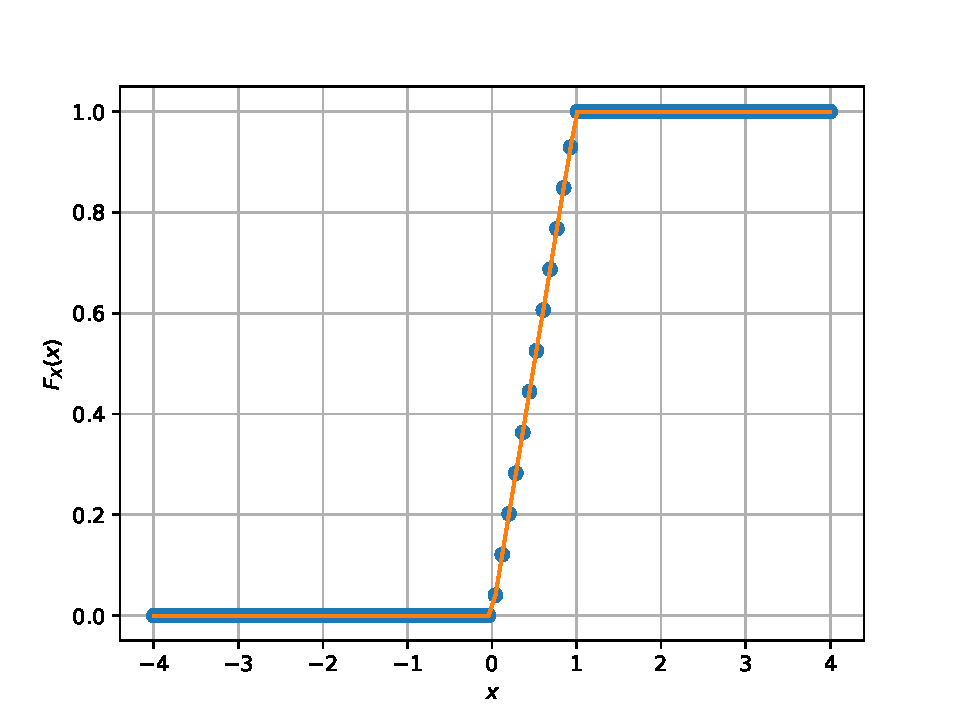
\includegraphics[width=\columnwidth]{../figs/uni_cdf.pdf}
	\caption{}
	\label{fig:1.3}
\end{figure}
%
\item
Find a theoretical expression for $F_{U}(x)$.

\solution 

Pdf of Uniform distribution between [0,1] is given by,
\begin{align}
    f_U(x) = \begin{cases}
        1, & x \in [0,1] \\
        0, & \text{otherwise}
    \end{cases}
\end{align}
\begin{align}
    F_U(x) = \int_{-\infty}^{x} f_U(x) dx
\end{align}
Case-1: x $<$ 0,
\begin{align}
    F_U(x) &= \int_{-\infty}^{x} 0 dx \\
    &= 0
\end{align}
Case-2: x $\in$ [0,1],
\begin{align}
    F_U(x) &= \int_{-\infty}^{0} 0 dx + \int_{0}^{x} 1 dx\\
    &= x
\end{align}\
Case-3: x $>$ 1,
\begin{align}
    F_U(x) &= \int_{-\infty}^{0} 0 dx + \int_{0}^{1} 1 dx + \int_{1}^{x} 0 dx\\
    &= 1
\end{align}
Hence,
\begin{align}
    F_U(x) = \begin{cases}
    0, & x < 0 \\
    x, & x \in [0,1] \\
    1, & x > 1
    \end{cases}
\end{align}
%
\item
The mean of $U$ is defined as
%
\begin{equation}
E\sbrak{U} = \frac{1}{N}\sum_{i=1}^{N}U_i
	\label{eq:mean-form}
\end{equation}
%
and its variance as
%
\begin{equation}
\text{var}\sbrak{U} = E\sbrak{U- E\sbrak{U}}^2 
	\label{eq:var-form}
\end{equation}
Write a C program to  find the mean and variance of $U$.

\solution 

Download the following files,
\begin{lstlisting}
wget https://github.com/Anshul-Sangrame/AI1110/blob/main/Assignment/solution/1/coeffs.h
wget https://github.com/Anshul-Sangrame/AI1110/blob/main/Assignment/solution/1/1_4.c
\end{lstlisting}
Execute the above files using code,
\begin{lstlisting}
gcc 1_4.c -lm
./a.out
\end{lstlisting}
The following result is obtained
\begin{align*}
    E\sbrak{U} &= 0.500007 \\
    \text{var}\sbrak{U} &= 0.083301
\end{align*}
%
\item Verify your result theoretically given that
\end{enumerate}
%
\begin{equation}
E\sbrak{U^k} = \int_{-\infty}^{\infty}x^kdF_{U}(x)dx
\end{equation}

\solution

$F_U(x)$ for uniform distribution,
\begin{align}
    F_U(x) = \begin{cases}
    0, & x < 0 \\
    x, & x \in [0,1] \\
    1, & x > 1
    \end{cases}
\end{align}
\begin{align}
    E[U] &= \int_{-\infty}^{\infty} x dF_U(x) \\
    &= \int_{-\infty}^{0} 0 dx + \int_{0}^{1} x dx + \int_{1}^{\infty} 0 dx \\
    \label{eq: U}
    &= \frac{1}{2}
\end{align}
\begin{align}
    E[U^2] &= \int_{-\infty}^{\infty} x^2dF_U(x) \\
    &= \int_{-\infty}^{0} 0 dx + \int_{0}^{1} x^2 dx + \int_{1}^{\infty} 0 dx \\
    \label{eq: U^2}
    &= \frac{1}{3}
\end{align}
\begin{align}
    E[U-E[U]]^2 &= E[U^2] - [E[U]]^2
\end{align}
From Equation \eqref{eq: U} and \eqref{eq: U^2},
\begin{align}
    E[U-E[U]]^2 &= \frac{1}{3} - \brak{\frac{1}{2}}^2 \\
    &= \frac{1}{3} - \frac{1}{4} \\
    &= \frac{1}{12} \approx 0.083
\end{align}
%
%
\section{Central Limit Theorem}
%
\begin{enumerate}[label=\thesection.\arabic*
,ref=\thesection.\theenumi]
%
\item
Generate $10^6$ samples of the random variable
%
\begin{equation}
X = \sum_{i=1}^{12}U_i -6
\end{equation}
%
using a C program, where $U_i, i = 1,2,\dots, 12$ are  a set of independent uniform random variables between 0 and 1
and save in a file called gau.dat

\solution

Download the following files,
\begin{lstlisting}
wget https://github.com/Anshul-Sangrame/AI1110/blob/main/Assignment/solution/1/coeffs.h
wget https://github.com/Anshul-Sangrame/AI1110/blob/main/Assignment/solution/2/2_1.c
\end{lstlisting}
Execute the above files using code,
\begin{lstlisting}
gcc 2_1.c -lm
./a.out
\end{lstlisting}
%
\item
Load gau.dat in python and plot the empirical CDF of $X$ using the samples in gau.dat. What properties does a CDF have?

\solution 

Download the following files,
\begin{lstlisting}
wget https://github.com/Anshul-Sangrame/AI1110/blob/main/Assignment/solution/2/2_2.py
\end{lstlisting}
Execute the above file using code,
\begin{lstlisting}
python3 2_2.py
\end{lstlisting}
Plot \ref{fig:2.2} obtained is symmetric about (0,0.5)
\begin{figure}[!ht]
	\centering
	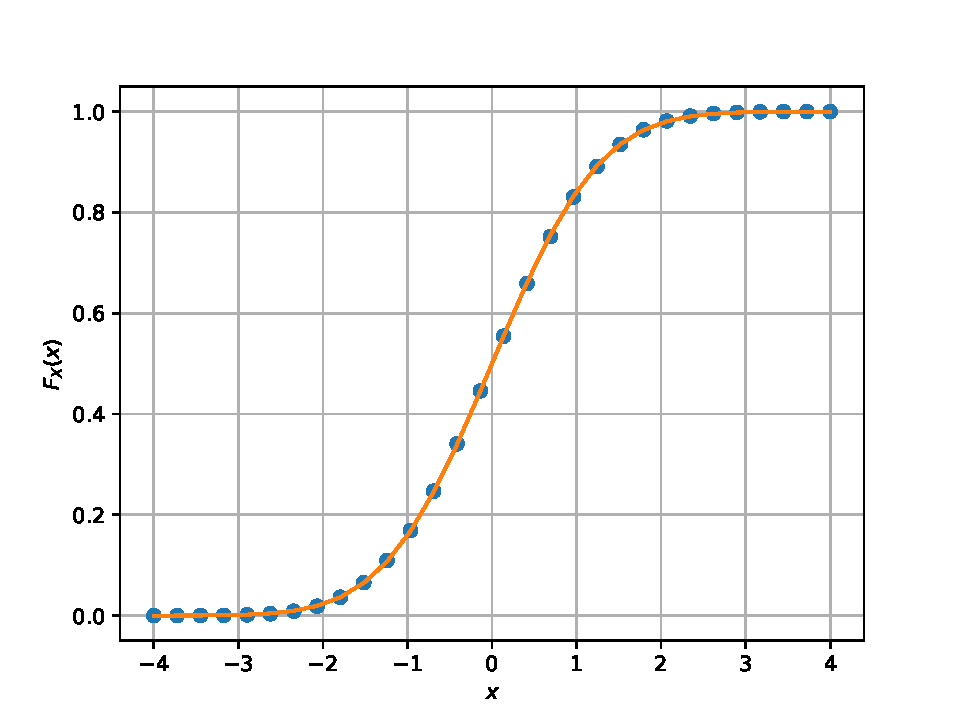
\includegraphics[width=\columnwidth]{../figs/gauss_cdf.pdf}
	\caption{}
	\label{fig:2.2}
\end{figure}
%
\item
Load gau.dat in python and plot the empirical PDF of $X$ using the samples in gau.dat. The PDF of $X$ is defined as
\begin{align}
p_{X}(x) = \frac{d}{dx}F_{X}(x)
	\label{eq:pdf-cdf}
\end{align}
What properties does the PDF have?

\solution 

Download the following files,
\begin{lstlisting}
wget https://github.com/Anshul-Sangrame/AI1110/blob/main/Assignment/solution/2/2_3.py
\end{lstlisting}
Execute the above file using code,
\begin{lstlisting}
python3 2_3.py
\end{lstlisting}
Plot \ref{fig:2.3} obtained is symmetric about y-axis
\begin{figure}[!ht]
    \centering
    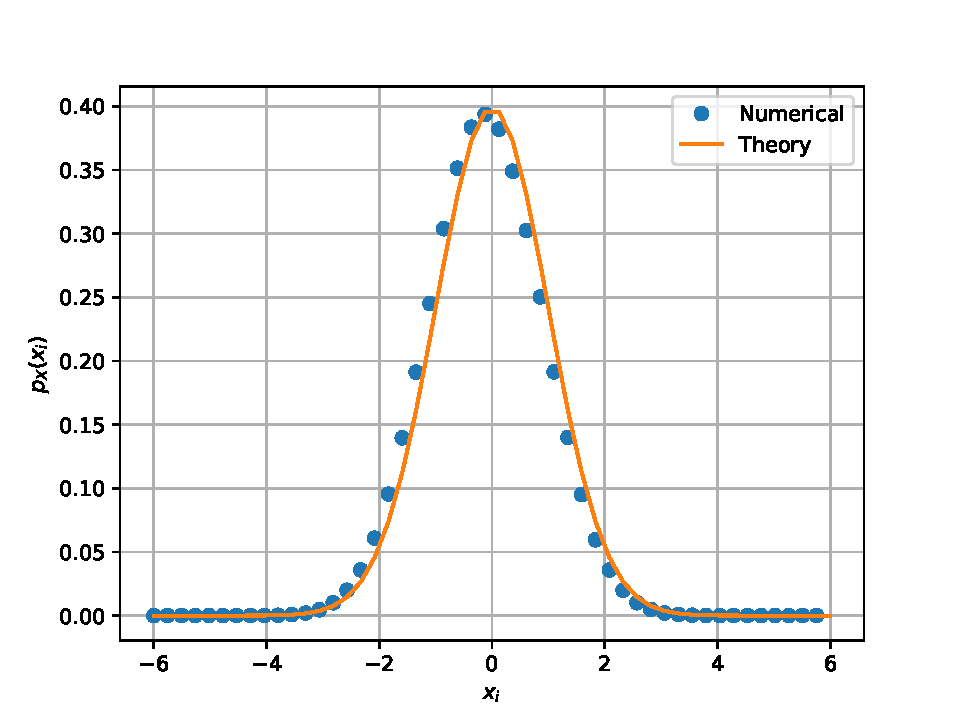
\includegraphics[width=\columnwidth]{../figs/gauss_pdf.pdf}
    \caption{}
    \label{fig:2.3}
\end{figure}
%
\item Find the mean and variance of $X$ by writing a C program.

\solution

Download the following files,
\begin{lstlisting}
wget https://github.com/Anshul-Sangrame/AI1110/blob/main/Assignment/soltion/1/coeffs.h
wget https://github.com/Anshul-Sangrame/AI1110/blob/main/Assignment/solution/2/2_4.c
\end{lstlisting}
Execute the above files using code,
\begin{lstlisting}
gcc 2_4.c -lm
./a.out
\end{lstlisting}
The result is,
\begin{align}
    E\sbrak{U} &= 0.000294 \\
    \text{var}\sbrak{U} &= 0.999561
\end{align}
%
\item Given that 
\begin{align}
p_{X}(x) = \frac{1}{\sqrt{2\pi}}\exp\brak{-\frac{x^2}{2}}, -\infty < x < \infty,
\end{align}
repeat the above exercise theoretically.

\solution

\begin{align}
E\sbrak{U} &= \int_{-\infty}^{\infty} up_X(u) du \\
\end{align}
$up_X(u)$ is a odd function.
\begin{align}
E\sbrak{U} &= 0 \\
\end{align}
\begin{align}
E\sbrak{U^2} &= \int_{-\infty}^{\infty} \frac{u^2}{\sqrt{2\pi}}\exp\brak{-\frac{u^2}{2}} du \\
&= \frac{1}{\sqrt{2\pi}} \int_{-\infty}^{\infty} u\brak{u\exp\brak{-\frac{u^2}{2}}}du
\end{align}
Using integration by parts,
\begin{align}
E\sbrak{U^2} &= -u\frac{1}{\sqrt{2\pi}}\exp{\brak{-\frac{u^2}{2}}}\Big|_{-\infty}^{\infty}  + \nonumber \\ 
& \int_{-\infty}^{\infty} \frac{1}{\sqrt{2\pi}}\exp\brak{-\frac{u^2}{2}}  \\ 
                &= 0 + \frac{1}{\sqrt{2\pi}}\sqrt{2\pi} \\
                &= 1
\end{align}
Hence,
\begin{align}
\text{var}\sbrak{U} &= E\sbrak{U^2} - \sbrak{E\sbrak{U}}^2 \\
&= 1
\end{align}
%
\end{enumerate}
\section{From Uniform to Other}
\begin{enumerate}[label=\thesection.\arabic*
,ref=\thesection.\theenumi]
%
\item
Generate samples of 
%
\begin{equation}
V = -2\ln\brak{1-U}
\end{equation}
%
and plot its CDF.
 
\solution

Download the following files,
\begin{lstlisting}
wget https://github.com/Anshul-Sangrame/AI1110/blob/main/Assignment/solution/coeffs.h
wget https://github.com/Anshul-Sangrame/AI1110/blob/main/Assignment/solution/3/3_1.c
wget https://github.com/Anshul-Sangrame/AI1110/blob/main/Assignment/solution/3/3_1.py
\end{lstlisting}
Execute the above files using code,
\begin{lstlisting}
gcc 3_1.c -lm
./a.out
python3 3_1.py
\end{lstlisting}
Plot \ref{fig:3.1} is obtained
\begin{figure}[!ht]
    \centering
    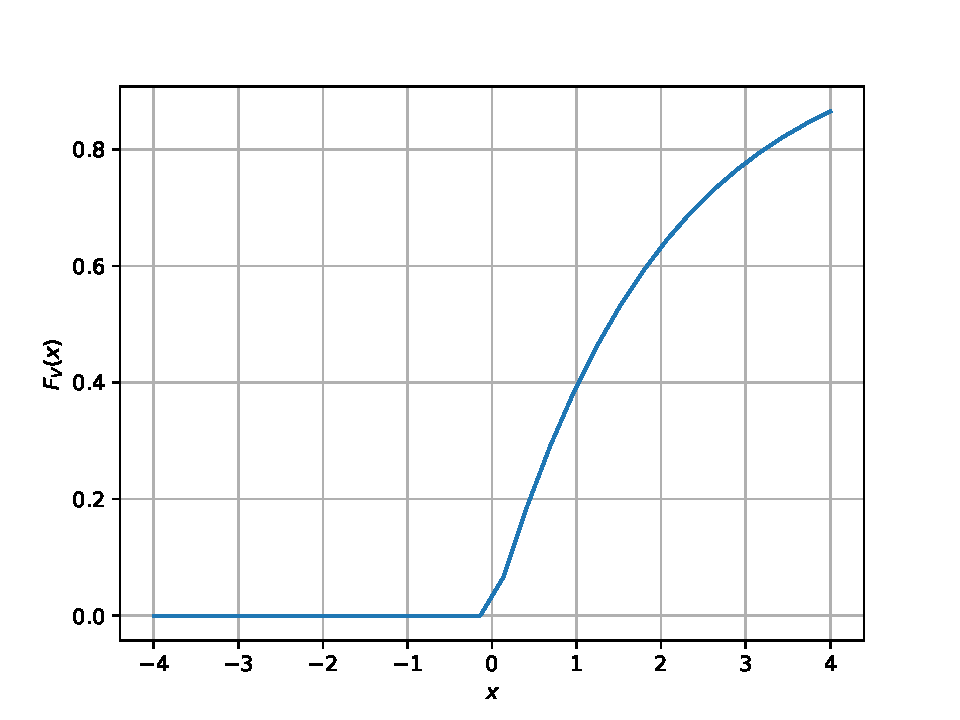
\includegraphics[width=\columnwidth]{../figs/V_cdf.pdf}
    \caption{}
    \label{fig:3.1}
\end{figure}
%
\item Find a theoretical expression for $F_V(x)$.

\solution

\begin{align}
    F_V(x) &= Pr\brak{V \leq x} \\
    &= Pr\brak{-2 \ln \brak{1-U} \leq x} \\
    &= Pr\brak{U \leq 1 - e^{-\frac{x}{2}}} \\
    F_V(x) &= F_U\brak{1 - e^{-\frac{x}{2}}} \\
    &= \begin{cases}
    0, & 1 - e^{-\frac{x}{2}}< 0 \\
    1 - e^{-\frac{x}{2}}, & 1 - e^{-\frac{x}{2}}\in [0,1] \\
    1, & 1 - e^{-\frac{x}{2}}> 1
    \end{cases}
\end{align}
Now,
\begin{align}
    1 - e^{-\frac{x}{2}} &< 0 \\
    \implies x &<0
\end{align}
\begin{align}
    0\leq1 - e^{-\frac{x}{2}} &\leq1 \\
    \implies x &\geq0
\end{align}
\begin{align}
    1<1 - e^{-\frac{x}{2}} \\
    \implies x \in \phi
\end{align}
Hence,
\begin{align}
    F_V(x) = \begin{cases}
    0, & x<0\\
    1 - e^{-\frac{x}{2}}, & x\geq0
    \end{cases}
\end{align}
%
%\item
%Generate the Rayleigh distribution from Uniform. Verify your result through graphical plots.
\end{enumerate}
\section{Triangular Distribution}
\begin{enumerate}[label=\thesection.\arabic*
,ref=\thesection.\theenumi]
\item Generate
	\begin{align}
		T = U_1 + U_2
	\end{align}
	
\solution

Download the following files,
\begin{lstlisting}
wget https://github.com/Anshul-Sangrame/AI1110/blob/main/Assignment/solution/coeffs.h
wget https://github.com/Anshul-Sangrame/AI1110/blob/main/Assignment/solution/4/4_1.c
\end{lstlisting}
Execute the above files using code,
\begin{lstlisting}
gcc 4_1.c -lm
./a.out
\end{lstlisting}
%
\item Find the CDF of $T$.

\solution

Download the following files,
\begin{lstlisting}
wget https://github.com/Anshul-Sangrame/AI1110/blob/main/Assignment/solution/4/4_2.py
\end{lstlisting}
Execute the above files using code,
\begin{lstlisting}
python3 4_2.py
\end{lstlisting}
Plot \ref{fig:4.2} is obtained
\begin{figure}[!ht]
    \centering
    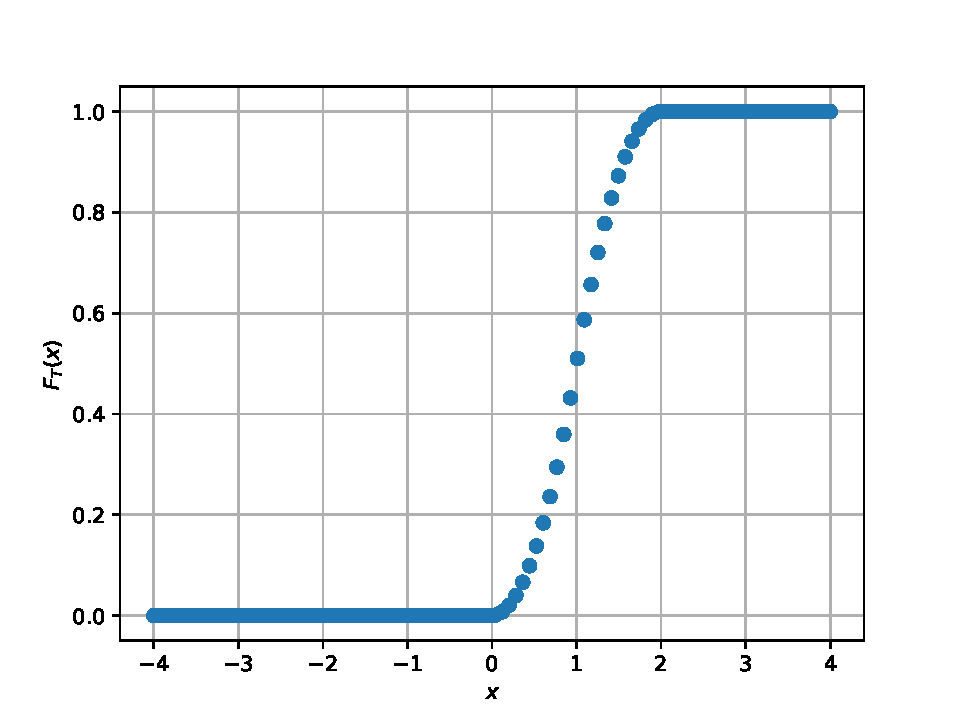
\includegraphics[width=\columnwidth]{../figs/tri_cdf_empirical.pdf}
    \caption{}
    \label{fig:4.2}
\end{figure}
%
\item Find the PDF of $T$.

\solution

Download the following files,
\begin{lstlisting}
wget https://github.com/Anshul-Sangrame/AI1110/blob/main/Assignment/solution/4/4_3.py
\end{lstlisting}
Execute the above files using code,
\begin{lstlisting}
python3 4_3.py
\end{lstlisting}
Plot \ref{fig:4.3} is obtained
\begin{figure}[!ht]
    \centering
    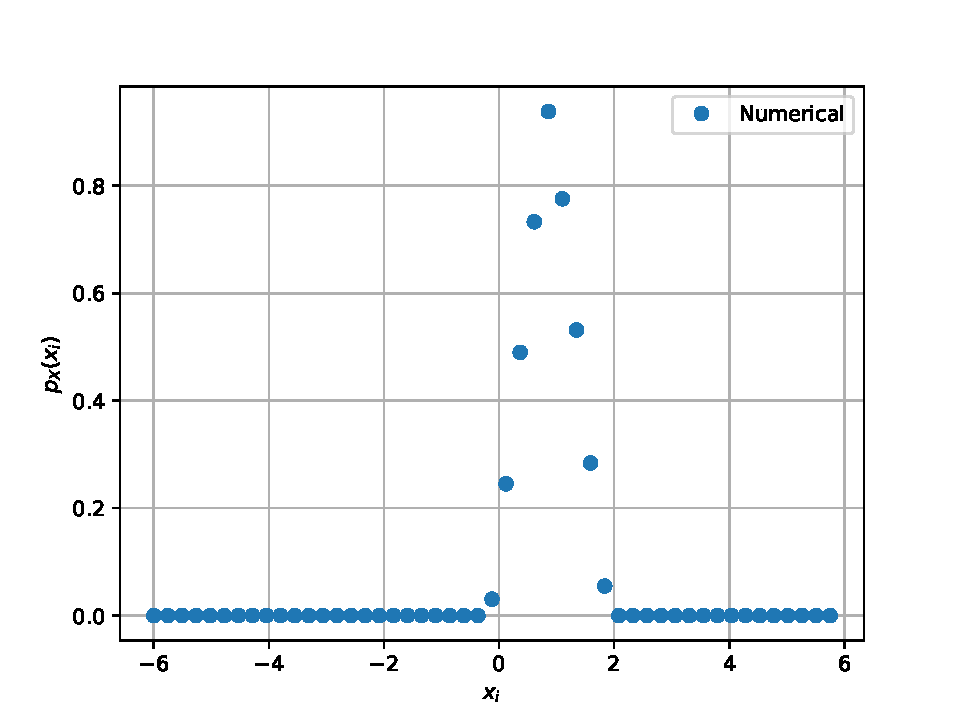
\includegraphics[width=\columnwidth]{../figs/tri_pdf_empirical.pdf}
    \caption{}
    \label{fig:4.3}
\end{figure}
%
\item Find the theoretical PDF and CDF of $T$.

\solution

The CDF of $T$ is given by
	\begin{align}
		F_T(t) = \pr{T \le t} = \pr{U_1 + U_2 \le t}	
	\end{align}		
	Since $U_1, U_2 \in [0,1] \implies U_1 + U_2 \in [0,2]$
	Therefore, if $t \ge 2$, then $U_1 + U_2 \le t$ is always true and if $t < 0$, then $U_1 + U_2 \le t$ is always false.
	
	Now, fix the value of $U_1$ to be some $x$
	\begin{align}
		x + U_2 \le t \implies U_2 \le t - x
	\end{align}
	
	If $0 \le t \le 1$, then $x$ can take all values in $[0,t]$
	\begin{align}
		F_T(t)	&= \int_0^t \pr{U_2 \le t - x} p_{U_1}(x) \der{x} \\
		&= \int_0^t F_{U_2}(t-x) p_{U_1}(x) \der{x}
	\end{align}
	\begin{align}
		0 \le x \le t &\implies 0 \le t - x \le t \le 1 \\
		&\implies F_{U_2}(t-x) = t - x
	\end{align}
	\begin{align}
		F_T(t) &= \int_0^t (t-x) \cdot 1 \cdot \der{x} \\
		&= \left. tx - \frac{x^2}{2} \right|_0^t \\
		&= \frac{t^2}{2}
	\end{align}
	
	If $1 < t < 2$, $x$ can only take values in $[0,1]$ as $U_1 \le 1$
	\begin{align}
		F_T(t)	&= \int_0^1 F_{U_2}(t-x) \cdot 1 \cdot \der{x} 
	\end{align}
	\begin{align}
		0 \le x \le t - 1 &\implies 1 \le t - x \le t \\
		t - 1 \le x \le 1 &\implies 0 < t - 1 \le t - x \le 1
	\end{align}
	\begin{align}
		F_T(t) &= \int_0^{t-1} 1 \der{x} + \int_{t-1}^1 (t-x)\der{x} \\
		&= t - 1 + t(1 - (t - 1)) - \frac{1}{2} + \frac{(t-1)^2}{2} \\
		&= t - 1 + 2t - t^2 -\frac{1}{2} + \frac{t^2}{2} + \frac{1}{2} - t \\ 
		&= -\frac{t^2}{2} + 2t - 1
	\end{align}
	
	Therefore,
	\begin{align}
		F_T(t) = 
		\begin{cases}
		0 & t < 0 \\
		\dfrac{t^2}{2} & 0 \le t \le 1 \\
		 2t -\dfrac{t^2}{2} - 1 & 1 < t < 2 \\
		1 & t \ge 2
		\end{cases}
	\end{align}
	
The PDF of $T$ is given by
	\begin{align}
		p_T(t) &= \frac{\der{}}{\der{t}} F_T(t) \\
		\therefore p_T(t) &=
		\begin{cases}
			0 & t < 0 \\
			t & 0 \le t \le 1 \\
			2 - t & 1 < t < 2 \\
			0 & t \ge 2
		\end{cases}
	\end{align}
%
\item Verify your results through a plot.

\solution

Download the following files,
\begin{lstlisting}
wget https://github.com/Anshul-Sangrame/AI1110/blob/main/Assignment/solution/4/4_5_1.py
wget https://github.com/Anshul-Sangrame/AI1110/blob/main/Assignment/solution/4/4_5_2.py
\end{lstlisting}
Execute the above files using code,
\begin{lstlisting}
python3 4_5_1.py
python3 4_5_2.py
\end{lstlisting}
Plot \ref{fig:4.5.1} is obtained is pdf
\begin{figure}[!ht]
    \centering
    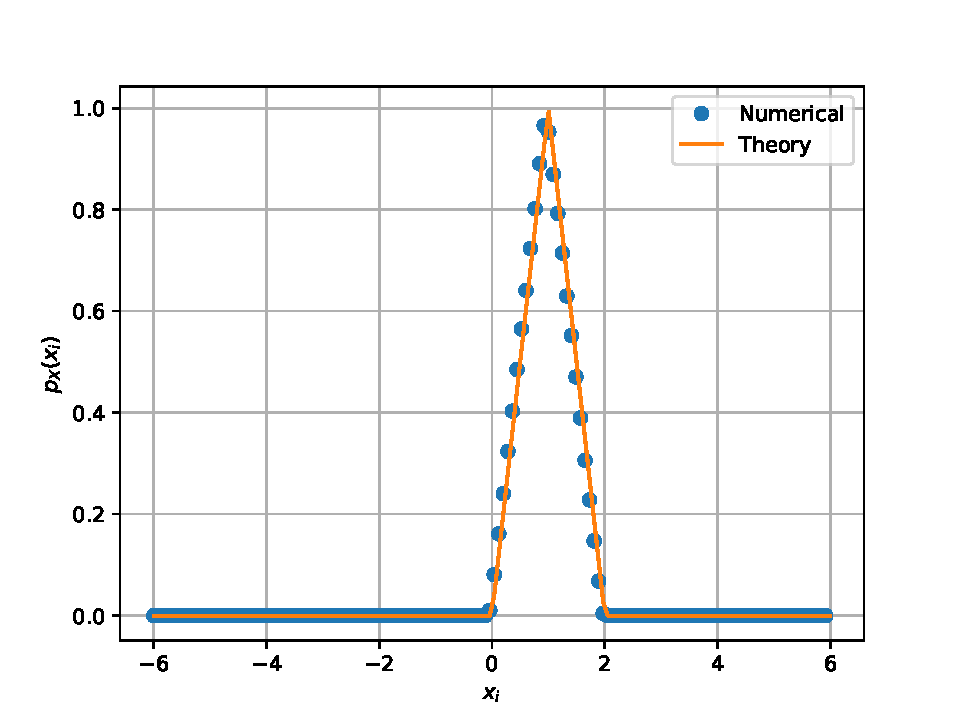
\includegraphics[width=\columnwidth]{../figs/tri_pdf.pdf}
    \caption{}
    \label{fig:4.5.1}
\end{figure}
Plot \ref{fig:4.5.2} is obtained is cdf
\begin{figure}[!ht]
    \centering
    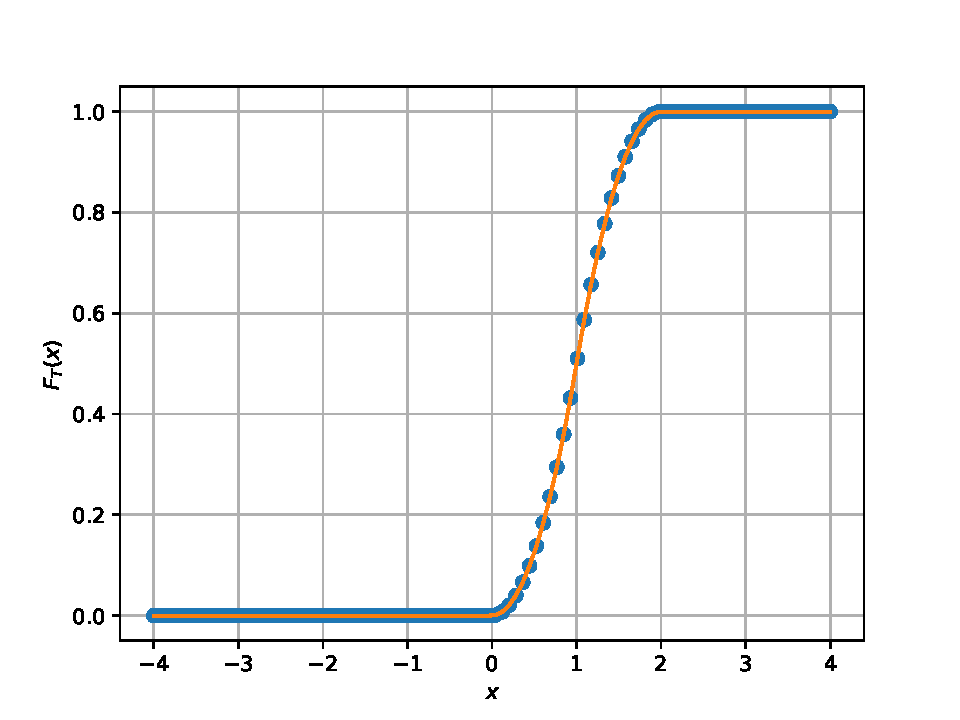
\includegraphics[width=\columnwidth]{../figs/tri_cdf.pdf}
    \caption{}
    \label{fig:4.5.2}
\end{figure}
\end{enumerate}
%
%
\section{Maximum Likelihood}
%
\begin{enumerate}[label=\thesection.\arabic*
,ref=\thesection.\theenumi]
%
\item Generate equiprobable $X \in \cbrak{1, -1}$.

\solution

Download the following files,
\begin{lstlisting}
wget https://github.com/Anshul-Sangrame/AI1110/blob/main/Assignment/solution/5/5.1.c
wget https://github.com/Anshul-Sangrame/AI1110/blob/main/Assignment/solution/coeffs.h
\end{lstlisting}
Execute the above files using code,
\begin{lstlisting}
gcc 5.1.c -lm
./a.out
\end{lstlisting}
%
\item Generate 
	\begin{align}
		Y = AX + N
	\end{align}
where $A  = 5 \text{ dB}, X \in \cbrak{1, -1}$ is Bernoulli and $N \sim \gauss{0}{1}$.

\solution

Download the following files,
\begin{lstlisting}
wget https://github.com/Anshul-Sangrame/AI1110/blob/main/Assignment/solution/5/5.2.c
wget https://github.com/Anshul-Sangrame/AI1110/blob/main/Assignment/solution/coeffs.h
\end{lstlisting}
Execute the above files using code,
\begin{lstlisting}
gcc 5.2.c -lm
./a.out
\end{lstlisting}
%
\item Plot Y using a scatter plot.

\solution

Download the following files,
\begin{lstlisting}
wget https://github.com/Anshul-Sangrame/AI1110/blob/main/Assignment/solution/5/5.3.py
\end{lstlisting}
Execute the above files using code,
\begin{lstlisting}
python3 5.3.py
\end{lstlisting}
Plot \ref{fig:5.2} is obtained
\begin{figure}[!ht]
    \centering
    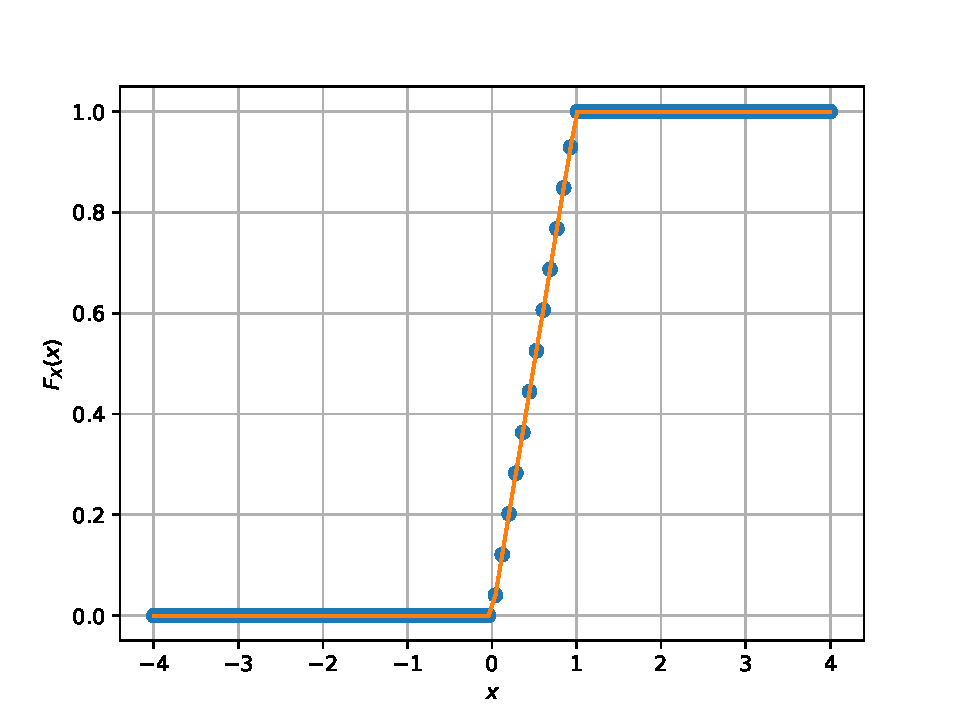
\includegraphics[width=\columnwidth]{../figs/uni_cdf.pdf}
    \caption{}
    \label{fig:5.2}
\end{figure}
%
\item Guess how to estimate $X$ from $Y$.

\solution

From the plot of $Y$, we see that the estimate model can be written as
\begin{align}
	\hat{X} = 
	\begin{cases}
		1 & Y > 0 \\
		0 & Y < 0
	\end{cases}
\end{align}
%
\item Find 
	\begin{align}
		P_{e|0} = \pr{\hat{X} = -1|X = 1}
	\end{align}
and
	\begin{align}
		P_{e|1} = \pr{\hat{X} = 1|X = -1}
	\end{align}
	
\solution

Letting $X = 1$ and $X = -1$ respectively, we see the number of mismatched data points to compute the error probabilities. The simulation is coded in
\begin{lstlisting}
wget https://github.com/Anshul-Sangrame/AI1110/blob/main/Assignment/solution/5/5.5.py
\end{lstlisting}
and can be run by typing
\begin{lstlisting}
python3 5.5.py
\end{lstlisting}
The results are
		\begin{align}
			P_{e|0} = 5.02 \times 10^{-4} \\
			P_{e|1} = 5.24 \times 10^{-4}
		\end{align}
%
\item Find $P_e$ assuming that $X$ has equiprobable symbols.

\solution

Here, $\pr{X = 1} = \pr{X = -1} = 0.5$. Thus,
	\begin{align}
		P_e &= \pr{X = 1}P_{e|1} + \pr{X = -1}P_{e|0} \label{eq:pe-gen} \\
		&= \frac{1}{2}\brak{P_{e|0} + P_{e|1}} = 5.13 \times 10^{-4}
	\end{align}
%
\item Verify by plotting the theoretical $P_e$ wrt $A$ from 0 dB to 10 dB.

\solution

\begin{align}
	P_{e|0} &= \pr{\hat{X} = 1 | X = -1}\\
	&= \pr{Y > 0 | X = -1} \\
	&= \pr{AX + N > 0 | X = -1} \label{eq:thresh} \\
	&= \pr{N > A} = \qfunc{A}
\end{align}
since $X$ and $N$ are independent. Writing a similar expression for $P_{e|1}$ and noting that 
\begin{align}
	\pr{N < -A} = \pr{N > A} = \qfunc{A}
\end{align}
it follows that $P_e = \qfunc{A}$. This is the idea used to plot the theoretical $P_e$. The plot is coded both in the rectangular axes and the semilog-y axes. Download the relevant codes using 
\begin{lstlisting}
wget https://github.com/Anshul-Sangrame/AI1110/blob/main/Assignment/solution/5/5.7.py
wget https://github.com/Anshul-Sangrame/AI1110/blob/main/Assignment/solution/5/5.7_semilog.py
\end{lstlisting}
Execute the above files using code,
\begin{lstlisting}
python3 5.7.py
python3 5.7_semilog.py
\end{lstlisting}
Plot \ref{fig:5.7} obtained in rectangular axis
\begin{figure}[!ht]
    \centering
    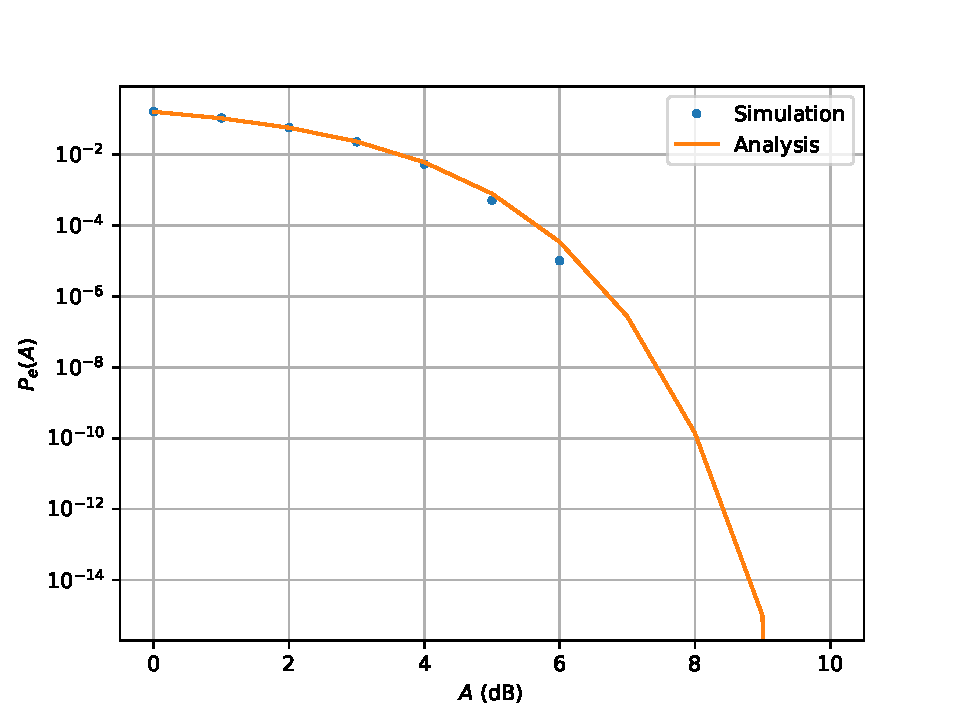
\includegraphics[width=\columnwidth]{../figs/5_6.pdf}
    \caption{}
    \label{fig:5.7}
\end{figure}

Plot \ref{fig:5.7_semilog} obtained in semilog-y axis
\begin{figure}[!ht]
    \centering
    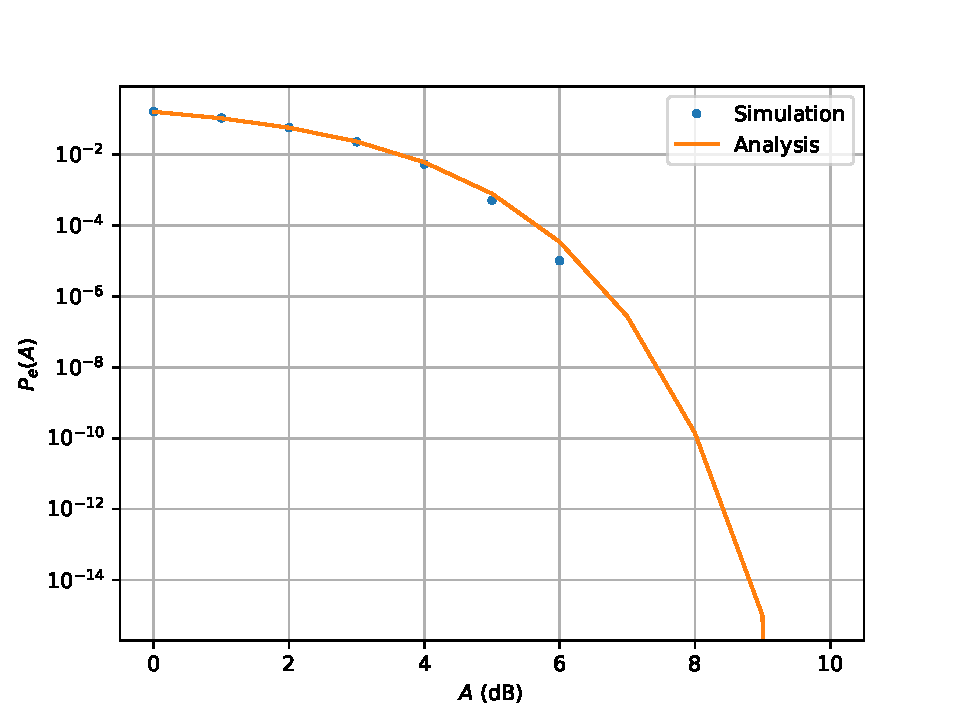
\includegraphics[width=\columnwidth]{../figs/5_6_semilog.pdf}
    \caption{}
    \label{fig:5.7_semilog}
\end{figure}
%
\item Now, consider a threshold $\delta$ while estimating $X$ from $Y$. Find the value of $\delta$ that maximizes the theoretical $P_e$.

\solution

To estimate $X$ from $Y$, we now consider the following:
\begin{align}
    X = 
    \begin{cases}
        1, & Y > \delta \\
        -1, & Y < \delta
    \end{cases}
\end{align}
Therefore,
\begin{align}
	P_e &= \pr{X = -1}\qfunc{A + \delta} \nonumber \\ 
	&+ \pr{X = 1}\qfunc{A - \delta} \label{eq:delta-gen} \\
	&= \frac{1}{2}\brak{\qfunc{A + \delta} + \qfunc{A - \delta}} 
	\label{eq:func-delta}
\end{align}
To minimise $P_e$, we differentiate the above equation wrt $\delta$:
\begin{align}
0 &= \frac{d}{d\delta} \left(\frac{1}{2}(Q_N(A - \delta) + Q_N(A + \delta))\right) \\
&= \frac{1}{2} (\frac{1}{\sqrt{2\pi}} e^{-\frac{(\delta - A)^2}{2}} - \frac{1}{\sqrt{2\pi}} e^{-\frac{(A + \delta)^2}{2}} ) \\
\intertext{Therefore,}
(\delta - A)^2 &= (\delta + A)^2 \\
\implies \delta &= 0
\end{align}
%
\item Repeat the above exercise when
\begin{align*}
	p_x(0) = p
\end{align*}

\solution

\begin{align}
    P_e &= P_{e|0} p+ P_{e|1} (1-p) \\
    &= p Q_N(A - \delta) + (1-p)Q_N(A + \delta)
\intertext{Differentiating as before, we get:}
0 &= p \frac{1}{\sqrt{2\pi}} e^{-\frac{(\delta - A)^2}{2}} - (1-p)\frac{1}{\sqrt{2\pi}} e^{-\frac{(A + \delta)^2}{2}} 
\end{align}
 Taking $\ln$ on both sides we have:
 \begin{align}
    \ln{p} - \frac{(\delta - A)^2}{2} &= \ln{1-p} - \frac{(\delta + A)^2}{2} \\
	\implies 2\delta A &= \ln{\frac{1-p}{p}} \\
    \implies \delta &= \frac{1}{2A} \ln{\frac{1-p}{p}}
 \end{align}
 %
\item Repeat the above exercise using the MAP criterion.

\solution

Using theorem of conditional probabilities,
\begin{align}
    p_{X|Y}(x|y) &= \frac{p_{Y|X}(y|x) \times p_X(x)}{p_Y(y)} \\
	p_{X|Y}(x|y) &= \frac{p_X(x)Pr(Ax + N = y)}{p_Y(y)} \\
	p_{X|Y}(x|y) &= \frac{p_X(x)Pr(N = y - Ax)}{p_Y(y)} \\
	p_{X|Y}(x|y) &= \frac{p_X(x)p_N(y - Ax)}{p_Y(y)} \\
	p_{X|Y}(x|y) &= \frac{\frac{1}{\sqrt{2\pi}}p_X(x)e^{-\frac{(y-Ax)^2}{2}}}{p_Y(y)} \\
\end{align}

When $X=1$, we have:
\begin{align}
    p_{X|Y}(1|y) &= \frac{p_{Y|X}(y|1) \times p_X(1)}{p_Y(y)} \\
    &= \frac{\left(1-p\right) \frac{e^{-\frac{(y-A)^2}{2}}}{\sqrt{2\pi}}}{ p \frac{e^{-\frac{(y+A)^2}{2}}}{\sqrt{2\pi}} + \left(1-p\right) \frac{e^{-\frac{(y-A)^2}{2}}}{\sqrt{2\pi}}} \\
    &= \frac{\left(1-p\right) e^{2yA}}{p + \left(1-p\right) e^{2yA}}
\end{align}

Similarly when $X=-1$,
\begin{align}
	p_{X|Y}(-1|y) &= \frac{p}{p + (1-p)e^{2yA}}
\end{align}

Therefore, when $ p_{X|Y}(1|y) >  p_{X|Y}(-1|y)$, we have:
\begin{align}
    \frac{\left(1-p\right) e^{2yA}}{p + \left(1-p\right) e^{2yA}} &> \frac{p}{p + \left(1-p\right) e^{2yA}} \\
    e^{2yA} &> \frac{p}{\left(1-p\right)} \\
    \label{eq:y-condition}
    y &> \frac{1}{2A} \ln{\frac{p}{\left(1-p\right)}}
\end{align}
Therefore, when Eq. \eqref{eq:y-condition}, we can assert that $X = 1$, and $X = -1$ otherwise.
\end{enumerate}
%
%
\section{Gaussian to Other}
%
\begin{enumerate}[label=\thesection.\arabic*,ref=\thesection.\theenumi]
%
\item Let $X_1 \sim  \gauss{0}{1}$ and $X_2 \sim  \gauss{0}{1}$. Plot the CDF and PDF of
%
\begin{equation}
V = X_1^2 + X_2^2
\end{equation}

\solution

Applying following transformation on $X_1$ and $X_2$,
\begin{align}
	X_1 = R\cos{\Theta} \\
	X_2 = R\sin{\Theta}
\end{align}
Where $R \in [0, \infty), \Theta \in [0, 2\pi)$. The Jacobian Matrix for this transformation is given by
		\begin{align}
			\mtx{J} &= \myvec{\pd{X_1}{R} & \pd{X_2}{R} \\
							 \pd{X_1}{\Theta} & \pd{X_2}{\Theta}} \\
					&= \myvec{\cos{\Theta} & \sin{\Theta} \\
							  -R\sin{\Theta} & R\cos{\Theta}} \\
			\implies |\mtx{J}| &= R
			\label{eq:Jacobian}
		\end{align}
We also know that
		\begin{align}
			|\mtx{J}|p_{X_1, X_2}(x_1, x_2) &= p_{R, \Theta}(r, \theta) \\
			\implies p_{R, \Theta}(r, \theta) &= Rp_{X_1}(x_1)p_{X_2}(x_2) \label{eq:iid-split} \\
			&= \frac{R}{2\pi}\exp{\brak{-\frac{X_1^2 + X_2^2}{2}}} \\
			&= \frac{R}{2\pi}\exp{\brak{-\frac{R^2}{2}}}
			\label{eq:joint}
		\end{align}
Where \eqref{eq:iid-split} follows as $X_1, X_2$ are iid random variables. Thus,
		\begin{align}
			p_R(r) &= \int_{0}^{2\pi}p_{R, \Theta}(r, \theta)d\theta \\
			&= R\exp{\brak{-\frac{R^2}{2}}}
		\end{align}
However, $V = X_1^2 + X_2^2 = R^2 \geq 0$, thus $F_V(x) = 0$. For $x < 0$,
		\begin{align}
			F_V(x) &= F_R(\sqrt{x}) \\ 
			&= \int_{0}^{\sqrt{x}}r\exp{\brak{-\frac{r^2}{2}}}dr \\
			&= \int_{0}^{\frac{x}{2}}e^{-t}dt = 1 - e^{-\frac{x}{2}}
		\end{align}
Where $t = \frac{r^2}{2}$ for $x \geq 0$, thus
		\begin{align}
			F_V(x) &= 
			\begin{cases}
				1 - e^{-\frac{x}{2}} & x \geq 0 \\
				0 & x < 0 
			\end{cases} \label{eq:chi-cdf} \\
			p_V(x) & = \frac{d F_V(x)}{dx}\\
			&= \begin{cases}
				0, & x < 0 \\
				\frac{1}{2}e^{-\frac{x}{2}}, & x \geq 0 \\
			\end{cases} \label{eq:chi-pdf}
		\end{align}
Download the following files to verify the plot,
\begin{lstlisting}
wget https://github.com/Anshul-Sangrame/AI1110/blob/main/Assignment/solution/6/6.1.c
wget https://github.com/Anshul-Sangrame/AI1110/blob/main/Assignment/solution/coeffs.h
wget https://github.com/Anshul-Sangrame/AI1110/blob/main/Assignment/solution/6/6.1.cdf.py
wget https://github.com/Anshul-Sangrame/AI1110/blob/main/Assignment/solution/6/6.1.pdf.py
\end{lstlisting}
Execute the programs using the code in terminal,
\begin{lstlisting}
gcc 6.1.c -lm
./a.out
python3 6.1.cdf.py
python3 6.1.pdf.py
\end{lstlisting}
Plot \ref{fig:6.1.cdf} is CDF
\begin{figure}[!ht]
    \centering
    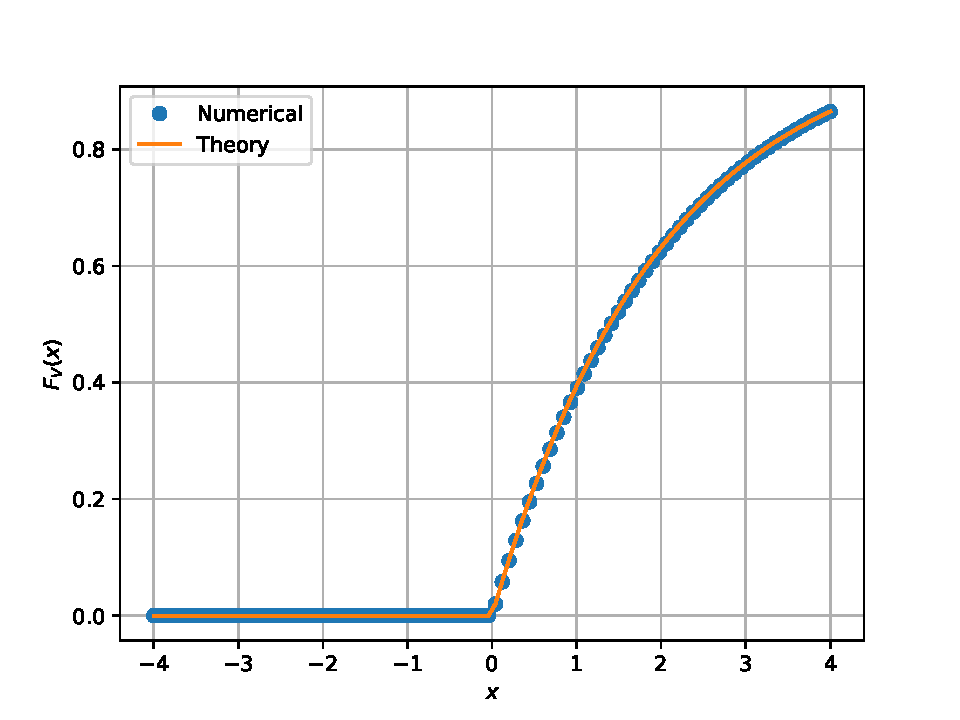
\includegraphics[width=\columnwidth]{../figs/chi_cdf.pdf}
    \caption{}
    \label{fig:6.1.cdf}
\end{figure}

Plot \ref{fig:6.1.pdf} is PDF
\begin{figure}[!ht]
    \centering
    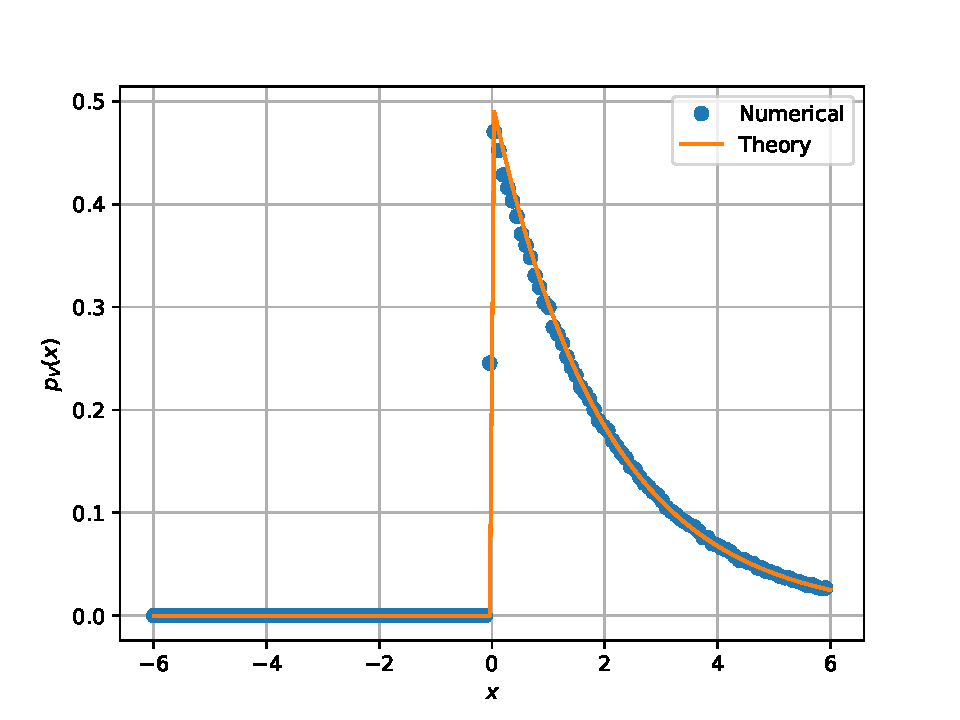
\includegraphics[width=\columnwidth]{../figs/chi_pdf.pdf}
    \caption{}
    \label{fig:6.1.pdf}
\end{figure}
%
\item If
\begin{align}
	F_V(x) = 
	\begin{cases}
		1 - e^{-\alpha x} & x \geq 0 \\
		0 & x < 0
	\end{cases}
\end{align}
find $\alpha$.

\solution

From \eqref{eq:chi-cdf}, $\alpha = 0.5$ 
%
\item Plot the CDF and PDF of 
\begin{align}
	A = \sqrt{V}
\end{align}

\solution

For $x \geq 0$,
\begin{align}
	F_A(x) &= \pr{A \leq x}\\
	F_A(x) &= \pr{\sqrt{V} \leq x}\\
	F_A(x) &= \pr{V \leq x^2} \\
	F_A(x) &= F_V(x^2)
\end{align}
From equation \eqref{eq:chi-cdf},
\begin{align}
	F_A(x) &= \begin{cases}
		0, & x < 0 \\
		1-e^{x^2/2}, & x \geq 0 \\
	\end{cases} \label{eq:ral-cdf} \\
	p_A(x) &= \frac{d F_V(x)}{dx}\\
	&= \begin{cases}
		0, & x < 0 \\
		xe^{-\frac{x^2}{2}}, & x \geq 0 \\
	\end{cases} \label{eq:ral-pdf}
\end{align}

Download the following files to verify the plot,
\begin{lstlisting}
wget https://github.com/Anshul-Sangrame/AI1110/blob/main/Assignment/solution/6/6.1.c
wget https://github.com/Anshul-Sangrame/AI1110/blob/main/Assignment/solution/coeffs.h
wget https://github.com/Anshul-Sangrame/AI1110/blob/main/Assignment/solution/6/6.1.cdf.py
wget https://github.com/Anshul-Sangrame/AI1110/blob/main/Assignment/solution/6/6.1.pdf.py
\end{lstlisting}
Execute the programs using the code in terminal,
\begin{lstlisting}
gcc 6.1.c -lm
./a.out
python3 6.1.cdf.py
python3 6.1.pdf.py
\end{lstlisting}
Plot \ref{fig:6.1.cdf} is CDF
\begin{figure}[!ht]
    \centering
    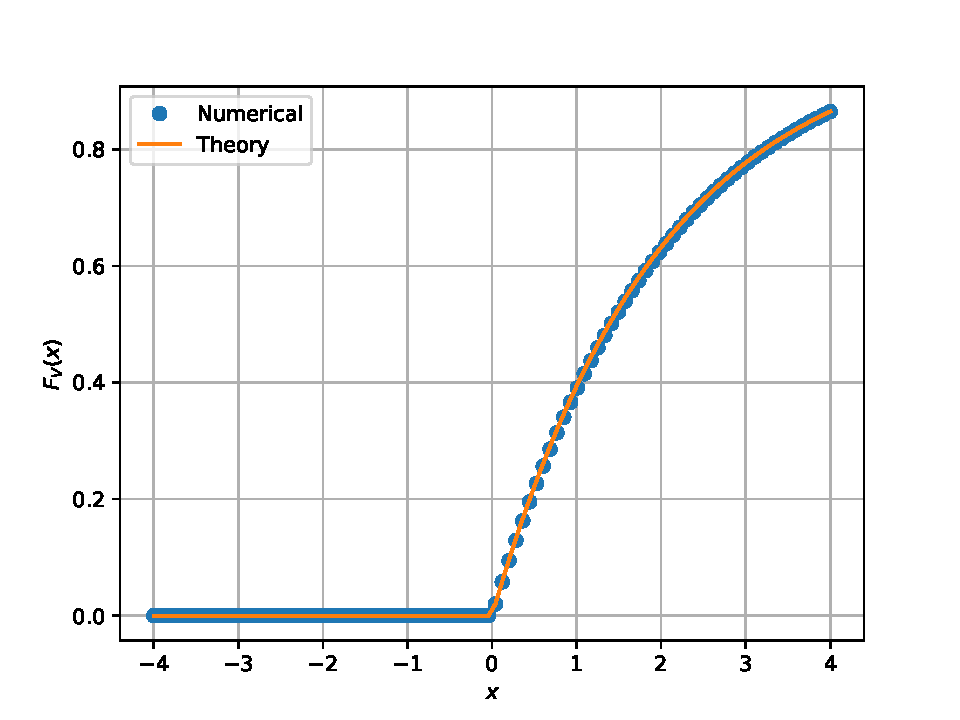
\includegraphics[width=\columnwidth]{../figs/chi_cdf.pdf}
    \caption{}
    \label{fig:6.1.cdf}
\end{figure}

Plot \ref{fig:6.1.pdf} is PDF
\begin{figure}[!ht]
    \centering
    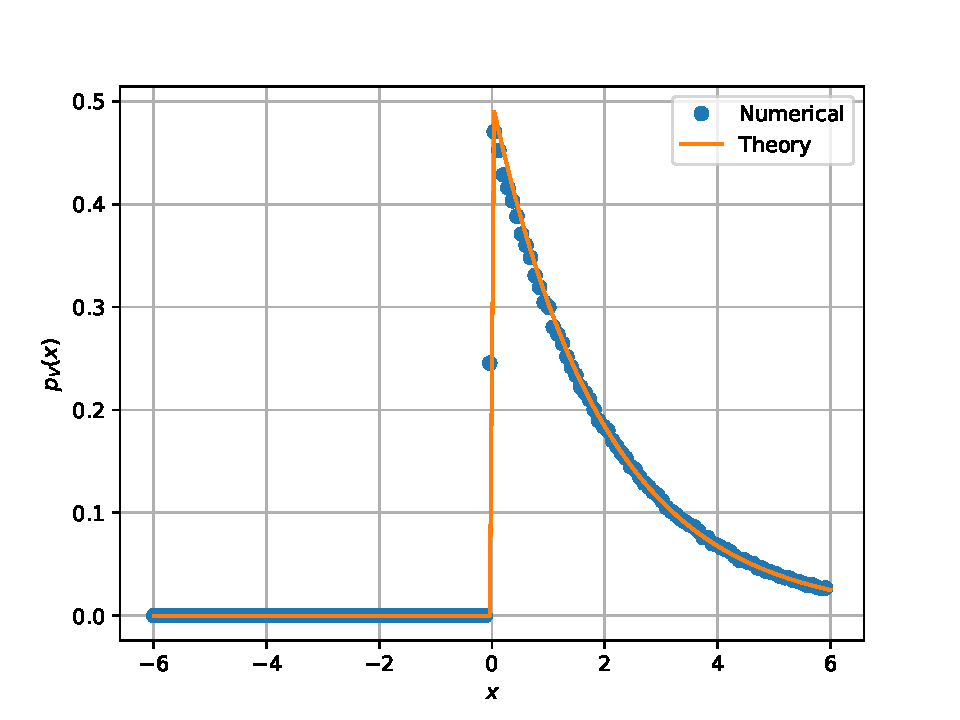
\includegraphics[width=\columnwidth]{../figs/chi_pdf.pdf}
    \caption{}
    \label{fig:6.1.pdf}
\end{figure}
%
\end{enumerate}
%
\end{document}